\documentclass[final]{article}

\usepackage[paperwidth=80cm,paperheight=120cm,margin=0cm]{geometry}
\usepackage{graphicx}
\usepackage{tikz}
\usepackage{tabularx}
\usepackage{booktabs}
\usepackage{array}
\usepackage{xcolor}
\usepackage{iftex}
\ifPDFTeX
  \usepackage[T1]{fontenc}
  \usepackage[utf8]{inputenc}
  \usepackage{helvet}
\else
  \usepackage{fontspec}
\fi
\usepackage{enumitem}
\usepackage{ragged2e}
\usepackage{eso-pic}
\usepackage{amsmath}

\ifPDFTeX
\else
  \setmainfont{Helvetica Neue}[
    BoldFont={Helvetica Neue Bold},
    ItalicFont={Helvetica Neue Italic}
  ]
  \setsansfont{Helvetica Neue}[
    BoldFont={Helvetica Neue Bold},
    ItalicFont={Helvetica Neue Italic}
  ]
\fi
\renewcommand{\familydefault}{\sfdefault}
\pagestyle{empty}
\setlength{\parindent}{0pt}

\definecolor{siiBlue}{HTML}{466DB4}
\definecolor{siiTeal}{HTML}{42B4B8}
\definecolor{ink}{HTML}{14213D}
\definecolor{muted}{HTML}{536171}
\definecolor{rule}{HTML}{BBCBE5}
\definecolor{paleBlue}{HTML}{EAF2FF}
\definecolor{paleTeal}{HTML}{E8F8F6}
\definecolor{paleWarn}{HTML}{FFF4E8}
\definecolor{green}{HTML}{16845F}
\definecolor{orange}{HTML}{D4742A}
\definecolor{red}{HTML}{B6423C}

\AddToShipoutPictureBG*{%
  \AtPageLowerLeft{%
    
\includegraphics[width=\paperwidth,height=\paperheight]{figures/poster_template_background.jpg}%
  }%
}

\setlist[itemize]{
  leftmargin=1.05em,
  itemsep=0.42cm,
  topsep=0.26cm,
  parsep=0cm
}

\newcommand{\BlockTitle}[1]{%
  {\fontsize{35}{41}\selectfont\bfseries\color{ink}#1}\par
  \vspace{0.26cm}
  {\color{rule}\rule{\linewidth}{1.9pt}}\par
  \vspace{0.62cm}
}

\newcommand{\PosterBlock}[2]{%
  \begin{minipage}[t]{\linewidth}
    \BlockTitle{#1}
    {\fontsize{24}{31}\selectfont\color{ink}\RaggedRight #2}
  \end{minipage}
}

\newcommand{\MetricCard}[4]{%
  \begin{tikzpicture}
    \node[
      rounded corners=3mm,
      draw=#4,
      line width=1.45pt,
      fill=#4!8,
      text width=#1,
      minimum height=10.5cm,
      inner xsep=0.85cm,
      inner ysep=0.78cm,
      anchor=north west
    ] at (0,0) {
      {\fontsize{64}{68}\selectfont\bfseries\color{#4}#2}\par
      \vspace{0.42cm}
      {\fontsize{20}{25}\selectfont\color{muted}#3}
    };
  \end{tikzpicture}
}

\newcommand{\Status}[2]{\textcolor{#1}{\textbf{#2}}}

\begin{document}

% Header: intentionally uses almost the full blue template band.
\begin{tikzpicture}[remember picture,overlay]
  \node[anchor=north west,text width=58.5cm,align=left] at ([xshift=17.0cm,yshift=-5.9cm]current page.north west) {%
    {\fontsize{62}{69}\selectfont\bfseries\color{white}
    Risk-Controlled\\[-0.05cm]
    Tower-Taking in 1v1 MOBA\\[-0.05cm]
    Reinforcement Learning}\par
    \vspace{0.84cm}
    {\fontsize{24}{30}\selectfont\color{white}
    PPO reward shaping, checkpoint selection, and evidence-driven evaluation for Honor of Kings 1v1}\par
    \vspace{0.62cm}
    {\fontsize{17}{21}\selectfont\color{white}
    Decision Machine Learning Project \quad | \quad v1.2a training analysis \quad | \quad Shanghai Innovation Institute}
  };
\end{tikzpicture}

% Body: starts at the white template area and deliberately fills it.
\vspace*{29.0cm}
\hspace*{4.8cm}
\begin{minipage}[t]{70.4cm}

{\fontsize{26}{33}\selectfont\color{ink}\RaggedRight
\textbf{Central claim.} v1.2a learned a markedly safer policy than v1.1, but the best checkpoint still does not match v1.1's tower-taking strength. The correct conclusion is not ``training finished'', but \textbf{step-15003 should enter the full matchup evaluation matrix}.}

\vspace{1.7cm}

\begin{minipage}[t]{21.8cm}
\PosterBlock{Research Problem}{
\textbf{Goal.} Train a PPO agent to turn local lane advantages into stable tower-taking wins in a long-horizon 1v1 MOBA environment.

\vspace{0.72cm}
\textbf{Core difficulty.} Immediate combat rewards can make the policy fight, trade, or dive, while the real objective is delayed: preserve enough safety to destroy the enemy tower.

\vspace{0.72cm}
\textbf{Hypothesis.} Terminal outcome reward, explicit tower-pressure terms, and tactical-window diagnostics should improve objective conversion. Unsafe-dive penalties should reduce death inflation without making the policy passive.
}

\vspace{2.05cm}

\PosterBlock{v1.2 Implementation}{
\begin{itemize}
  \item \textbf{PPO backbone:} clipped policy loss, value loss, entropy regularization, GAE, legal-action masking, and gradient clipping.
  \item \textbf{Tower objective:} enemy tower damage, self tower damage, tower destroy, terminal win/loss, and timeout tower-gap rewards.
  \item \textbf{Tactical window:} push-window tower-damage reward plus zero-weight diagnostics.
  \item \textbf{Risk control:} death, unsafe-dive, and unsafe-dive severity penalties.
  \item \textbf{Evidence chain:} checkpoint, lineup, matchup, opponent source, terminal outcome, and reward-detail logging.
\end{itemize}

\vspace{0.65cm}
\[
R_t=\sum_i w_i\Delta f_i(s_t)+20R_{\mathrm{win}}+8R_{\mathrm{tower\ gap}}
\]
}

\vspace{2.05cm}

\PosterBlock{Acceptance Gates}{
\begin{tabularx}{\linewidth}{>{\raggedright\arraybackslash}X>{\raggedright\arraybackslash}X}
\toprule
\textbf{Gate} & \textbf{Target}\\
\midrule
Win rate & Beat 0.84, or match it with much lower death\\
Tower pressure & Enemy tower HP below 1400.59\\
Death control & Average death below 3.09\\
Coverage & All 9 hero matchups with side swaps\\
Diagnostics & Push-window share and unsafe-dive correlation\\
\bottomrule
\end{tabularx}
}
\end{minipage}
\hfill
\begin{minipage}[t]{22.4cm}
\BlockTitle{Best Candidate}
\begin{minipage}[t]{10.75cm}
\MetricCard{9.15cm}{0.78}{common-AI win rate at step-15003}{siiBlue}
\end{minipage}
\hfill
\begin{minipage}[t]{10.75cm}
\MetricCard{9.15cm}{0.47}{average deaths, far below v1.1 late 3.09}{green}
\end{minipage}

\vspace{1.65cm}

{\fontsize{24}{31}\selectfont\color{ink}\RaggedRight
\textbf{Checkpoint ranking selected step-15003.} It is the only checkpoint with both high win rate and strong objective pressure. Later checkpoints improve scalar reward but regress on gameplay metrics.}

\vspace{1.85cm}

\PosterBlock{Checkpoint Ranking}{
\begin{tabularx}{\linewidth}{r r r r r}
\toprule
\textbf{Step} & \textbf{Win} & \textbf{Enemy HP} & \textbf{Death} & \textbf{Score}\\
\midrule
15003 & 0.78 & 2129 & 0.47 & 75.79\\
17617 & 0.53 & 4106 & 0.53 & 48.50\\
15977 & 0.53 & 3978 & 0.69 & 48.35\\
10004 & 0.53 & 4735 & 0.59 & 47.66\\
17022 & 0.47 & 5423 & 0.56 & 41.09\\
\bottomrule
\end{tabularx}

\vspace{0.72cm}
\textbf{Selection rule.} Do not pick the final checkpoint by default. Use win rate, tower HP, death, and matchup evidence.
}

\vspace{2.05cm}

\PosterBlock{v1.2a vs. v1.1 Peak}{
\begin{tabularx}{\linewidth}{>{\raggedright\arraybackslash}X r r r}
\toprule
\textbf{Metric} & \textbf{v1.2a} & \textbf{v1.1} & \textbf{Delta}\\
\midrule
Win rate & 0.78 & 0.84 & -0.06\\
Enemy tower HP & 2129 & 1401 & +729\\
Self tower HP & 4296 & 7745 & -3449\\
Frame & 15726 & 13670 & +2055\\
Kill & 3.44 & 3.75 & -0.31\\
Death & 0.47 & 2.72 & -2.25\\
Money/frame & 0.53 & 0.58 & -0.05\\
Hero damage & 1.63 & 1.88 & -0.25\\
\bottomrule
\end{tabularx}

\vspace{0.72cm}
\textbf{Interpretation.} Safety improved dramatically, but objective conversion is weaker and slower.
}
\end{minipage}
\hfill
\begin{minipage}[t]{21.8cm}
\PosterBlock{Training Dynamics}{
\begin{itemize}
  \item \textbf{0-2979:} cold start; enemy tower HP remains above 9500.
  \item \textbf{4028-7018:} first breakthrough; win rate reaches 0.47.
  \item \textbf{7992-13964:} plateau around 0.38-0.53 win rate.
  \item \textbf{15003:} narrow peak with 0.78 win rate and 2129 enemy tower HP.
  \item \textbf{15977-17617:} reward improves, but gameplay metrics regress.
\end{itemize}

\vspace{0.72cm}
Win rate tracks tower pressure, self-tower survival, economy, kills, and outgoing hero damage. Death is no longer the main bottleneck because v1.2a has already compressed deaths into a low range.
}

\vspace{2.05cm}

\PosterBlock{Candidate Gate}{
\begin{tabularx}{\linewidth}{>{\bfseries}l X}
\toprule
\Status{green}{PASS} & death control; hero-damage balance; explicit checkpoint selection\\
\Status{orange}{WARN} & win rate below 0.84; tower pressure below v1.1 peak\\
\Status{red}{MISSING} & 9-matchup matrix, worst-matchup gap, push-window share, unsafe-dive correlation, death p90, self-tower p10, timeout rate\\
\bottomrule
\end{tabularx}

\vspace{0.72cm}
\textbf{Meaning.} The gate failure is actionable: run the missing evidence package before making a final v1.2 claim.
}

\vspace{2.05cm}

\PosterBlock{Next Experiment}{
\begin{itemize}
  \item Freeze \textbf{step-15003} as the v1.2a candidate.
  \item Run 9 hero matchups, side swaps, 20 repeats, and the planned skill grid.
  \item Preserve reward-detail logs for push-window and unsafe-dive analysis.
  \item Keep risk shaping, but increase tower-damage and terminal-win alignment.
  \item Compare v1.2, no-window, no-terminal, and death-only-risk ablations.
\end{itemize}
}
\end{minipage}

\vspace{1.85cm}

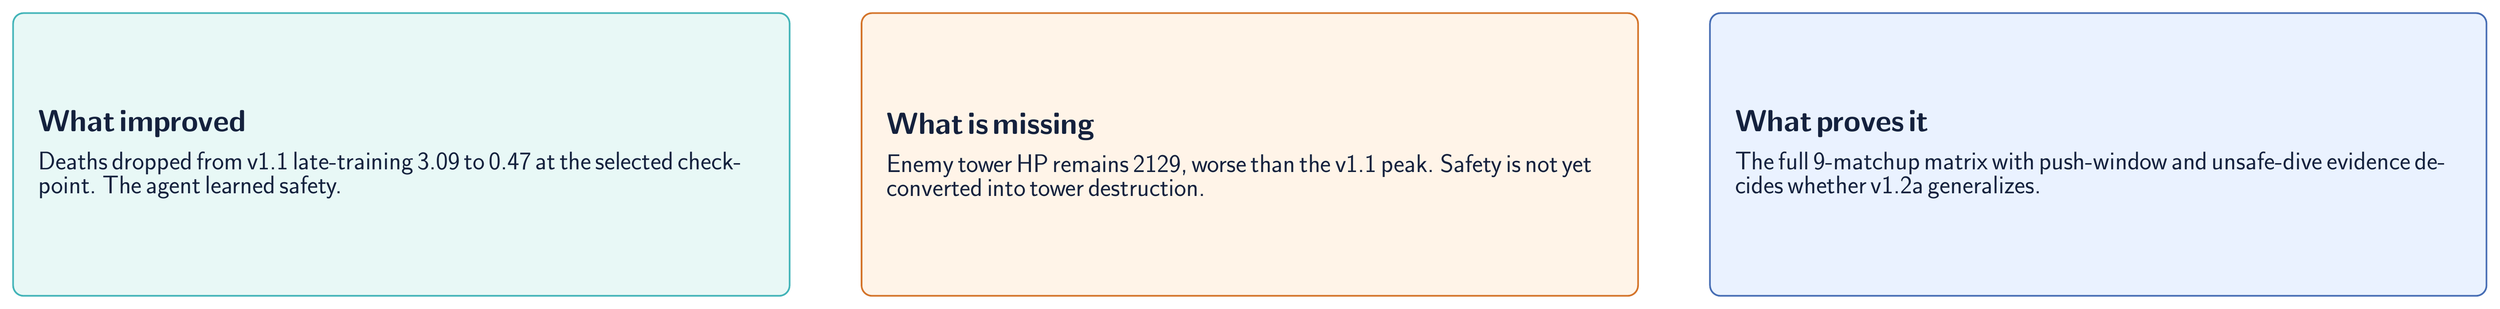
\begin{tikzpicture}
\node[
  rounded corners=3mm,
  fill=paleTeal,
  draw=siiTeal,
  line width=1.35pt,
  text width=20.8cm,
  minimum height=8.1cm,
  inner xsep=0.72cm,
  inner ysep=0.62cm,
  anchor=north west
] at (0,0) {
  {\fontsize{25}{30}\selectfont\bfseries\color{ink}What improved}\par
  \vspace{0.38cm}
  {\fontsize{20}{25}\selectfont\color{ink}
  Deaths dropped from v1.1 late-training 3.09 to 0.47 at the selected checkpoint. The agent learned safety.}
};
\node[
  rounded corners=3mm,
  fill=paleWarn,
  draw=orange,
  line width=1.35pt,
  text width=20.8cm,
  minimum height=8.1cm,
  inner xsep=0.72cm,
  inner ysep=0.62cm,
  anchor=north west
] at (24.3,0) {
  {\fontsize{25}{30}\selectfont\bfseries\color{ink}What is missing}\par
  \vspace{0.38cm}
  {\fontsize{20}{25}\selectfont\color{ink}
  Enemy tower HP remains 2129, worse than the v1.1 peak. Safety is not yet converted into tower destruction.}
};
\node[
  rounded corners=3mm,
  fill=paleBlue,
  draw=siiBlue,
  line width=1.35pt,
  text width=20.8cm,
  minimum height=8.1cm,
  inner xsep=0.72cm,
  inner ysep=0.62cm,
  anchor=north west
] at (48.6,0) {
  {\fontsize{25}{30}\selectfont\bfseries\color{ink}What proves it}\par
  \vspace{0.38cm}
  {\fontsize{20}{25}\selectfont\color{ink}
  The full 9-matchup matrix with push-window and unsafe-dive evidence decides whether v1.2a generalizes.}
};
\end{tikzpicture}

\vspace{1.2cm}

\begin{tikzpicture}
\node[
  rounded corners=3mm,
  fill=paleBlue,
  draw=siiBlue,
  line width=1.4pt,
  text width=69.0cm,
  inner xsep=0.95cm,
  inner ysep=1.05cm,
  anchor=north west
] at (0,0) {
  {\fontsize{38}{45}\selectfont\bfseries\color{ink}Takeaway}\par
  \vspace{0.52cm}
  {\fontsize{25}{32}\selectfont\color{ink}
  v1.2a shows that risk-aware reward shaping can sharply reduce deaths, but stable MOBA success still depends on converting safety into tower destruction. The next decisive evidence is the full matchup matrix for step-15003.}
};
\end{tikzpicture}

\end{minipage}

\begin{tikzpicture}[remember picture,overlay]
  \node[anchor=south west,text width=70.0cm,align=left] at ([xshift=4.9cm,yshift=2.25cm]current page.south west) {%
    {\fontsize{13.5}{17}\selectfont\color{white}
    Sources: \texttt{logs/v1.2a/summary.csv}, \texttt{logs/v1.2a/checkpoint\_ranking.md}, \texttt{logs/v1.2a/candidate\_gate.md}, \texttt{logs/v1.2/baseline\_v1.1.json}, and implemented v1.2 PPO reward/workflow code.}
  };
\end{tikzpicture}

\end{document}
